\chapter{Background}\label{C:backgroundsurvey}
This chapter introduces concepts which are used to motivate and develop the solution presented.

\section{Interpretability}
To create a system that is interpretable it is necessary to have an understanding of what it means to interpret a model, and how its interpretation might be evaluated. Interpretability of Machine Learning systems has been defined as \textit{"the ability to explain or to present in understandable terms"} \cite{doshi2017towards} which is ambiguous.\\

When is an interpretable model necessary? \cite{doshi2017towards} In some problem domains there is less risk associated with incorrect answers. An ANN which controls a virtual car has a low risk as poor or dangerous driving will only affect an artificial environment. Problem domains where there is a high risk associated with incorrect answers include Safety and Ethics. A survey, "Concrete Problems in AI Safety" \cite{amodei2016concrete} provides an example of potential safety issues with AI in the context of a cleaning robot.  For example, if the robot's objective is to have an environment containing no mess, how can the robot be prevented from disabling its sensors which it uses to detect the mess? Alternatively, a self-driving car might be penalized for running a stop light, but what is to prevent it from disabling the sensors that detect stop lights?\\

It has been demonstrated that Machine Learning systems learn human-like biases from textual data \cite{caliskan2017semantics}. A study done in 2010 \cite{ruggieri2010data} developed a method to analyze datasets for prejudices against particular classes of people. An analysis of the \textit{German Credit Dataset} was conducted. It which showed that discriminatory patterns were hidden in the data. An ANN trained on this data could learn these underlying biases. If the model was interpretable, then it could be examined for discriminatory patterns.\\

If an ANN model is presented as being interpretable how can this be verified scientifically? There are three categories of evaluation techniques \cite{doshi2017towards}.
\begin{enumerate}
	\item \textit{"Application-Grounded Evaluation"} Conducting experiments with human subjects in a specific problem domain. If the goal is to learn an interpretable classifier that grants bank loans, then a domain expert in granting/denying loans should be used to establish interpretability.
	
	\item \textit{"Human-Grounded Metrics"} Designing simpler experiments which still allow for establishing interpretability in a specific domain. This situation occurs when access to domain experts is either too expensive or difficult. The tasks can be simplified to allow humans that are not domain experts to complete them.
	
	\item \textit{"Functionally-Grounded Evaluation"} If it is possible to define interpretability of the problem then it can be used to establish this property in the model.
\end{enumerate}


\section{Rule Extraction}

A survey in 1995 focuses on rule extraction algorithms \cite{andrews1995survey}, identifying the reasons for needing these algorithms along with introducing ways to classify and compare them.\\

There are three categories that rule extraction algorithms fall into \cite{andrews1995survey}. An algorithm in the \textbf{decompositional} class focuses on extracting rules from each hidden/output unit. If an algorithm is in the \textbf{pedagogical} category, then rule extraction is thought of as a learning process. The ANN is treated as a black box, and the algorithm learns a relationship between the input and output vectors. The third category, \textbf{eclectic}, is a combination of decompositional and pedagogical. An eclectic, algorithm inspects the hidden/output neurons individually but extracts rules which represent the ANN globally \cite{tickle1998truth}.\\

To further divide the categories two more distinctions are introduced. One measures the portability of rule extraction techniques, i.e., how easily can they be applied to different types of ANN's? The second is criteria to assess the quality of extracted rules; these are accuracy, fidelity, consistency, and comprehensibility \cite{andrews1995survey}.

\begin{enumerate}
\item A rule set is \textbf{Accurate} if it can generalize, i.e., classify previously unseen examples.
\item The behavior of a rule set with high \textbf{fidelity} is close to that of the ANN from which it was extracted.
\item A rule set is \textbf{consistent} if when trained under different conditions it generates rules which assign the same classifications to unseen examples.
\item The measure of \textbf{comprehensibility} is defined by the number of rules in the set and the number of literals per rule.
\end{enumerate}

These surveys provide a framework for evaluating the rules extracted using a particular technique. By introducing this content, the reader is familiar with this approach to evaluating extracted rule sets. The solution developed in this report allows for rule exaction in some situations and will be assessed against these criteria. 

\section{LIME: Local Interpretable Model-Agnostic Explanations}
The paper "'Why should I Trust You?' Explaining the Predictions of Any Classifier" \cite{ribeiro2016should} published in 2016 presents a novel approach to the interpretation of Machine Learning models. The motivation for this research is the idea of trusting the answers provided, either in the context of an individual prediction or the model as a whole. The LIME technique explains  a single prediction. Trust in the model can be developed by inspecting explanations of many individual predictions.\\

Essentially the LIME algorithm treats the classifier as a black-box and generates many examples by slightly perturbing the instance for which an explanation is wanted and asks the model for a classification. It then constructs a linear model of local region around the instance using the classifications of the perturbed examples. A more detailed explanation of LIME is beyond the scope of this report.

LIME is a recent method for interpreting machine learning models. Consequently, it will provide a comparison point when evaluating the solution presented in this report.

\section{Noisy Neurons} \label{sec:background-noisy-neurons}
In 2016 the concept of Noisy-OR and Noisy-AND neurons \cite{LearningLogicalActivations} was presented. These neurons are based on the discrete boolean OR and AND gates. The motivation for this work was that logical functions are directly interpretable as functions of their input. Consequently, if a problem had a natural, logical decomposition, then it could be learned by Artificial Neural Networks using Noisy neurons.

\noindent
\begin{minipage}[t]{0.6\textwidth}
\vspace{0px}
The Noisy-OR neuron is derived from the Noisy-OR relation \cite{russell1995modern}, a concept in Bayesian Networks developed by Judea Pearl. A Bayesian Network represents the conditional dependencies between random variables in the form of a directed acyclic graph \cite{neapolitan2004learning}. Figure \ref{fig:bayesian-network-example} is a Bayesian network. It demonstrates the dependency between random variables "Rush Hour", "Raining", "Traffic", and "Late To Work". The connections between random variables show their dependencies, i.e., Traffic influences whether someone is late to work, and it being rush hour or raining influences whether there is traffic.\\

Consider a Bayesian Network consisting of a node $D$ with parents $S_1,..., S_n$. In other words, $D$ is dependent on each $S_i$. $S_i$ is independent from $S_j$ if $i \neq j$. The relationship between D and its parents is defined as if $S_1\ OR\ ...\ OR\ S_n$ is true then $D$ is true.\\
\end{minipage}
\hspace{0.05\textwidth}
\begin{minipage}[t]{0.35\textwidth}
\vspace{0px}
\begin{figure}[H]
	\centering
	\begin{minipage}[b]{1.0\textwidth}
		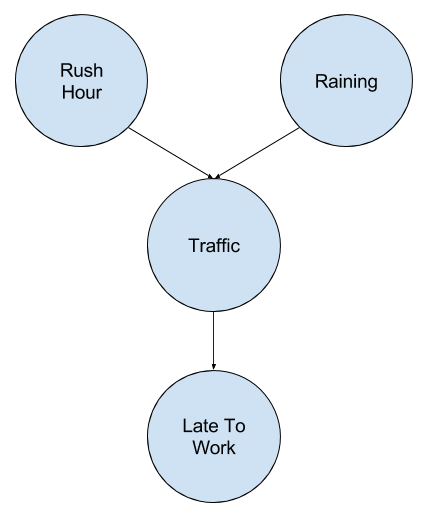
\includegraphics[width=\textwidth]{bayesian-network-example.png}
		\caption{}
		\label{fig:bayesian-network-example}
	\end{minipage}
	\hfill
\end{figure}
\end{minipage}

This relationship is binary, but there might be some uncertainty as to whether each $S_i$ influences $D$. Let $\epsilon_i$ be the probability that if $S_i = 1$ then $D = 0$, i.e. $P(D = 0|S_i = 1) = \epsilon_i$. Then $P(D = 0 | S_i = 1\ \forall i) = P(D = 0 | S_1 = 1) \cdot \cdot \cdot P(D = 0 | S_n = 1) = \prod_{i=1}^{n} \epsilon_i$. Therefore $P(D = 1| S_1 = 1, , S_n = 1)$ can be expressed as Equation \ref{equ:noisy-or-relation}.

\begin{align}
P(D = 1 | S_1 = 1, ..., S_n = 1) = 1 - \prod^n_{i=1} \epsilon_i
\label{equ:noisy-or-relation}
\end{align}

Equation \ref{fig:bayesian-network-example} is the noisy or relation. Consider the entended situation where $D$ has a belief that each $S_i$ is True. In the context of a neuron consider the inputs $x_1, ..., x_n$ to represent $D$'s belief of the probability that the inputs $1, ..., n$ are True. The output of a neuron as conditionally dependent on its inputs, each input node is a parent of the neuron.  $\epsilon_i$ is $D$'s uncertainty as to whether $x_i$ influences its output. The probability of $D$ being True is influenced by $x_i$ and $\epsilon_i$. A function $f$ is needed to compute the irrelevance of node $i$ in light of $x_i$ and $\epsilon_i$. The list in Figure \ref{fig:irelevence-function-cond} gives three desirable properties of $f(x_i, \epsilon_i)$ \cite{LearningLogicalActivations}.\\

\begin{figure}[H]
\begin{enumerate}
	\item $\epsilon = 1$ means that $f(\epsilon, x) = 1$. If $\epsilon = 1$, then the node does not influence the neuron. Consequently, it makes sense that the probability of irrelevance is 1.
	\item $x = 0$ means that $f(\epsilon, x) = 1$. If the neuron believes that the input node is off, then it makes sense for the probability of irrelevance to be 1.
	\item Monotonically increasing in $\epsilon$ and decreasing in x. In other words, fixing $x$ results in a function that monotonically increases as $\epsilon$ get closer to 1. Fixing $\epsilon$ results in a function that monotonically decreases as $x$ approaches 1. As the belief that the node is on increases, then the probability of relevance should decrease. Alternatively, as the neurons belief that the node has no influence increases, its probability of irrelevance should increase
\end{enumerate}
\caption{Three properties of the function $f$}
\label{fig:irelevence-function-cond}
\end{figure}

If the inputs of $f$ are restricted to be either 0 or 1 then it becomes apparent that properties (1) - (3) describe the logic function $x \implies \epsilon$ ($x$ implies $\epsilon$) , this is shown in Figure \ref{fig:f-actually-implies}. 

\noindent
\begin{minipage}[t]{0.5\textwidth}
\begin{figure}[H]
\begin{enumerate}
\item \textit{f(1,1) = 1:} This is shown by (1)
\item \textit{f(1,0) = 1:} Shown by (2)
\item \textit{f(0,1) = 0:} Fix $x = 1$ and let $\epsilon = 1$, $f(1,1) = 1$. As $\epsilon \rightarrow 0 $ $f$ is monotonically decreasing so $f(0,1) = 0$.
\item \textit{f(0,0) = 1:} Shown by (2)
\end{enumerate}
\caption{Demonstration that $f$ is the boolean function $x \implies \epsilon$ when $x,\epsilon \in \{0, 1\}$}
\label{fig:f-actually-implies}
\end{figure}
\end{minipage}
\hspace{0.05\textwidth}
\begin{minipage}[t]{0.45\textwidth}
\begin{figure}[H]
\begin{align*}
f(1,1) &= 1^1 = 1\\
f(1,0) &= 1^0 = 1\\
f(0,1) &= 0^1 = 0\\
f(0,0) &= 0^0 = 1\\
\end{align*}
\caption{Checking $f(\epsilon, x) = \epsilon^x$ is a Boolean Like Implies function. Note that for $f(0,0) = 0^0$ strictly this is undefined, but $\lim_{\epsilon \rightarrow 0} \epsilon^0 = 0$\\}
\label{fig:f-check-implies}
\end{figure}
\end{minipage}

A function $g(x_1, ..., x_m)$ is defined to be \textit{Boolean-Like} \cite{williams1986logic} when $x_i \in \{0, 1\} \forall i$ then $g(x_1, ..., x_m) \in \{0, 1\}$. Consequently, on top of properties (1) - (3) $f$ should be a \textit{boolean like} Implies function. A choice of $f$ which satisfies properties (1) - (3) is $f(x, \epsilon) = \epsilon^x$. It is a simple task to check that $f$ is a \textit{boolean like} Implies function. Figure \ref{fig:f-check-implies} shows that all properties are satisfied.


This choice of $f$ is not a unique solution, but it has a property which becomes convenient later on, specifically $\log(f) = \log(\epsilon^x) = x \cdot \log(\epsilon)$.

\begin{definition}
	A \textbf{Noisy-OR} Neuron has weights $\epsilon_1, ..., \epsilon_n \in (0,1]$ which represent the uncertainty that corresponding inputs $x_1, ..., x_n \in [0,1]$ influence the output. The activation of a Noisy-OR Neurons is given in Equation \ref{equ:noisy-or-activation-1}.
	
	\begin{align}
	a = 1 - \prod^p_{i=1} (\epsilon_i^{x_i})
	\label{equ:noisy-or-activation-1}
	\end{align}
\end{definition}

Consider that the Noisy-OR activation just defined is a \textit{boolean like} OR function. How can Equation \ref{equ:noisy-or-activation-1} be transformed to give a Noisy-AND activation which is \textit{boolean like}. From logic it is known that $a \land b = \lnot (\lnot a \lor \lnot b)$. Considering that $f_{NOT}(a) = 1 - a$ is a \textit{boolean like} NOT function then $f_{AND}(x_1, ..., x_n) = f_{NOT}(f_{OR}(f_{NOT}(x_1), ..., f_{NOT}(x_1)))$. Using this as intuition the Noisy-OR activation can be converted into a Noisy-AND.

\begin{definition}
	A \textbf{Noisy-AND} Neuron has weights $\epsilon_1, ..., \epsilon_n \in (0, 1]$ which represent the uncertainty that corresponding inputs $x_1, ..., x_n \in [0,1]$ influence the output. The activation of a Noisy-AND Neurons is given in Equation \ref{equ:noisy-and-activation-1}
	
	\begin{align}
	a = \prod^p_{i=1} (\epsilon_i^{1 - x_i})
	\label{equ:noisy-and-activation-1}
	\end{align}
\end{definition}

The noisy neurons are the building blocks for the two network architectures present in this report. Without an understanding of these concepts, it would be difficult to understand the motivations for the solution developed.

\section{Logical Normal Form Networks}
\subsection{CNF \& DNF}
A boolean formula is in Conjunctive Normal Form (CNF) if and only if it is a conjunction (and) of clauses. A clause in a CNF formula is given by a disjunction (or ) of literals. A literal is either an atom or the negation of an atom, and an atom is one of the variables in the formula.\\

Consider the boolean formula $\lnot a \lor (b \land c)$, then the CNF is $(\lnot a \lor b) \land (\lnot a \lor c)$. In this CNF formula the clauses are $(\lnot a \lor b)$, $(\lnot a \lor c)$, the literals used are $\lnot a$, $b$, $c$ and the atoms are $a$, $b$, $c$.\\

A boolean formula is in Disjunctive Normal Form (DNF) if and only if it is a disjunction (or) of clauses. A DNF clause is a conjunction (and) of literals. Literals and atoms are defined the same as in CNF formulas.\\

Consider the boolean formula $\lnot a \land (b \lor c)$, then the DNF is $(\lnot a \land b) \lor (\lnot a \land c)$.\\

\subsection{CNF \& DNF from Truth Table} \label{subsec:construct-cnfdnf}
Given a truth table representing a boolean formula, constructing a DNF formula involves taking all rows which correspond to True and combining them with an OR operation. To construct a CNF one combines the negation of any row which corresponds to False by an OR operation and negates it.

\begin{theorem}
	The maximum number of clauses in a CNF or DNF formula is $2^n$
	\label{thm:max-clause-cnfdnf}
\end{theorem}

\begin{proof}
	Assume the goal is to find the CNF and DNF for a Boolean formula B of size $n$, for which the complete truth table is given. The truth table has precisely $2^n$ rows.\\
	
	First, assume a CNF is being constructed, this is achieved by taking the OR of the negation of all rows corresponding to False, the NOT operation leaves the number of clauses unchanged. At most, there can be $2^n$ rows corresponding to False. Consequently, there is no more than $2^n$ clauses in the CNF.\\
	
	A similar argument shows that the same holds for DNF.
\end{proof}

\subsection{Definition of Logical Normal Form Networks}
In 1996 a class of networks called Logical Normal Form Networks \cite{herrmann1996backpropagation} (LNFNs) where developed. Focusing on learning the underlying CNF or DNF for a boolean expression which describes the problem. The approach relies on a specific network configuration along with restriction the function space of each neuron, allowing them to only perform an OR or AND on a subset of their inputs. Such OR and AND neurons are called Disjunctive and Conjunctive retrospectively. If the trained network can achieve a low enough error rate, then rules can be extracted from the network as a Boolean CNF or DNF expression \cite{herrmann1996backpropagation}.\\

The algorithm which extracts rules from LNFNs would be Electic and indeed is not Portable as the algorithm is specific to the LNFN architecture. It is not possible to further classify the rule extraction algorithm as the research developing it lacks any experimental results. Justification is also missing making the LNFNs challenging to reproduce.

\section{Logical Neural Networks}
Artificial Neural Networks (ANN's) consisting of Noisy-OR and Noisy-AND neurons are called Logical Neural Networks \cite{LearningLogicalActivations} (LNN's). If the network consists of only Noisy neurons then it a pure LNN. ANNs containing a mix of logical and standard activations where shown not to yield interpretable models, and also have lower performance. Consequently, when LNNs are referred to it will always be in the context of Pure LNNs.


\section{Learning Fuzzy Logic Operations in Deep Neural Networks}
A paper published in September 2017 \cite{godfrey2017parameterized} has a novel approach to combine Deep Learning and Fuzzy Logic. The goal of this paper is creating artificial neural networks which can be trained using backpropagation and be more interpretable. They propose a single activation which can learn to perform many different fuzzy logic operations. The result of this paper is a neural network architecture that can perform well as a classifier but also yield a model from which fuzzy rules can be extracted. The Fuzzy Logic networks where compared against standard deep neural networks (that used a \textit{tanh} activation function). In this comparison, they were found to have equivalent performance in some cases but worse in others. After training it was possible to extract fuzzy rules from the networks which were unable to perform well but had a simple representation. Fuzzy Logic Networks are a different approach to solving the problem outlined in this report. Consequently, they will be an interesting comparison point for the solution developed here.

